\documentclass[12pt,a4paper,oneside]{NITR}

\usepackage[hyphens]{url} 
%\usepackage[usenames,dvipsnames]{color}
%\usepackage[colorlinks=true,breaklinks,backref=true,linkcolor={MidnightBlue},citecolor={Fuchsia},urlcolor={OliveGreen}]{hyperref}
\usepackage[none]{hyphenat}
\usepackage{amsmath,amsfonts,mathdots,amssymb,yfonts}
\usepackage{graphicx}
\usepackage{tikz}
\usetikzlibrary{trees,shapes}
\usepackage{booktabs}
\usepackage{algorithm}
\usepackage{algorithmic}
%\usepackage{subfigure}
%\usepackage[ruled,linesnumbered,slide,vlined]{algorithm2e}
%\usepackage{verbatim}
%\usepackage{wrapfig}
%\usepackage{multirow}
%% % % % % % %
\onehalfspacing
\begin{document}
\sloppy
% % % % % % % % % % % % % % % % % % % % % % % % % % %
% % % % % % % % % % % % % % % % % % % % % % % % % % %
\author{Koshal Kumar Garg}
\rollNumber{114CS0100}
\authorGender{male}		%%Author's gender: male or female
\department{Department of Computer Science and Engineering}
\docTitle{Anomaly Detection in Streaming Data}

% % % % % % % % % % % % % % % % % % % % % % % % % % % % % %
% % % % % % % % % % % % % % % % % % % % % % % % % % % % % %
% % % Use any ONE of the following three as appropriate

%%\studentType{doctoral}			
%%\studentType{postgraduate}	
\studentType{undergraduate}
	
% % % % % % % % % % % % % % % % % % % % % % % % % % % % % %
% % % Use any ONE of the following as appropriate

%%\degree{Doctor of Philosophy} 				 %%Doctor of Philosophy; 
%%\degree{Master of Arts}					 %%Master of Arts;
%%\degree{Master of Technology}				 %%Master of Technology;
\degree{Bachelor of Technology}			 %%Bachelor of Technology;
%%\degree{Master of Business Administration} %%Master of Business Administration;

% % % % % % % % % % % % % % % % % % % % % % % % % % % % % %
% % % % % % % % % % % % % % % % % % % % % % % % % % % % % %

% % % Mention the discipline in which the degree is awarded
\degreeIn{Computer Science and Engineering}		

% % % Mention the specialization with which the degree is awarded. 
% %\specialization{Information Security}	

% % % % % % % % % % % % % % % % % % % % % % % % % % % % % %
% % % % % % % % % % % % % % % % % % % % % % % % % % % % % %

\docType{2}		%%Dissertation=1; Thesis=2; Project=3; Synopsis=4; Registration Report=5

% % % % % % % % % % % % % % % % % % % % % % % % % % % % % %
% % % % % % % % % % % % % % % % % % % % % % % % % % % % % %

\numOfSupervisors{1}

\principalSupervisor{Bidyut Kumar Patra}	%%Name only
%%\coSupervisor{Homi Jehangir Bhabha}			%%Name only
%%\firstMemberDSC{Carl Friedrich Gauss}		%%Name only
%%\secondMemberDSC{Isaac Newton}				%%Name only
%%\thirdMemberDSC{Dennis Ritchie}				%%Name only
%%\externalExaminer{Niels Bohr}				%%Name only
%%\chairperson{Aryabhata}						%%Name only
%%\hod{Varahamihira}							%%Name only

\principalSupervisorDesignation{Associate Professor}
%%\coSupervisorDesignation{Associate Professor}

% % % % % % % % % % % % % % % % % % % % % % % % % % % % % %
% % % % % % % % % % % % % % % % % % % % % % % % % % % % % %

\setDate{14}
\setMonth{May}
\setYear{2018}

% % % % % % % % % % % % % % % % % % % % % % % % % % % % % %
% % % % % % % % % % % % % % % % % % % % % % % % % % % % % %

\Font{1}	%% Times New Roman=1; Arial=2;
\setFont

% % % % % % % % % % % % % % % % % % % % % % % % % % % % % %
% % % % % % % % % % % % % % % % % % % % % % % % % % % % % %
% % % These may be used to fine tune the cover and title pages

\titlePageLineSpacing{2}
\titleWidth{.75}
\titleCoordinateX{0.16}
\titleCoordinateY{0.12}

% % % % % % % % % % % % % % % % % % % % % % % % % % %
% % % % % % % % % % % % % % % % % % % % % % % % % % %
% % % % % % % % % % % % % % % % % % % % % % % % % % %
	% %Fill details in "FrontPages.tex"
% % % % % % % % % % % % % % % % % % % % % % % % % % %
% % % % % % % % % % % % % % % % % % % % % % % % % % %
%%\coverPageSynReg		% %Needed for Synopsis Cover Page or 
						% %Registration Report Cover Page.
						% %To be used along with "\docType()".
						% %Use "\section{Introduction}\label{Guidelines}
Submission of synopsis or extended abstract is one of the mandatory requirements before submitting a doctoral or master thesis. It is not just a longer version of an abstract. It is as good as a research paper that conveys the essence of the thesis without overlooking the importance of introduction and conclusion. A synopsis should include the following~\textemdash~
\begin{itemize}
	\item Introduction
	\item Aim
	\item Method
	\item Results
	\item Conclusion
	\item Limitations
	\item References
	\item Dissemination
\end{itemize}

\noindent A synopsis is a self-contained, capsule description of the thesis that must make sense all by itself. Typical length of a synopsis should be between 5 and 10. Pages must of A4 dimension with 25mm margin on all four sides. The entire dissertation must be written using only a single font including all the texts inside graphs, figures, block diagrams, etc. While writing captions of tables and figures, the font size should be decreased by one point. Similarly, the font size of bibliography and index should also be lessened by a point. Students are advised to use the following in the body text~\textemdash
\begin{itemize}
\item[] serif fonts like Times New Roman (TNR) of size 12pt \\
or \\
\textsf{sans-serif fonts like Arial of size 11pt}. 
\end{itemize}
Needless to say that the use of font should be uniform throughout. Headings, Titles \textit{etc.} should use fonts as given below in Table~\ref{tab-fonts}.
{
\linespread{1}
\begin{table}[h]
\centering
\caption{Font sizes to be used in the dissertation}
\begin{tabular}{l C{25mm} C{25mm} c} 
\toprule
{Item} & Arial & {TNR} & {Justification}\\
\midrule\midrule
Main Text & 11 normal & 12 normal & Justified \\
\midrule
Sub-sub Heading & 11 bold & 12 bold & Left \\
\midrule
Sub Heading & 13 bold & 14 bold & Left \\
\midrule
Heading$^{\#}$ & 16 bold & 17 bold & Left \\
\midrule
Chapter Title & 22 bold & 24 bold & Center \\
\midrule
Chapter Number & 16 bold & 17 bold & Left \\
\bottomrule
\multicolumn{4}{l}{$^{\#}$Add serial number with one decimal place.} 
\end{tabular}
\label{tab-fonts}
\end{table}
}
\par The class file \texttt{NITR.cls} can be used to prepare a synopsis. One needs to invoke the statement ``\texttt{\textbackslash synopsisCoverPage}'' in the main ``\texttt{.tex}'' file with ``\texttt{\textbackslash docType(4)}'' and all necessary data in the ``\texttt{FrontPages.tex}''. The text of the synopsis can be written in ``\texttt{./SynopsisText/SynopsisText.tex}''."
						% %Comment rest.
\coverPage
\titlePage
%%\certificateOfExamination

\certificateOneSupervisor		%% Comment any
%%\certificateTwoSupervisors		%% one of these two

\dedication
\declaration
\acknowledgment
\abstract
% % % % % % % % % % % % % % % % % % % % % % % % % % %
% % % % % % % % % % % % % % % % % % % % % % % % % % %
\tableofcontents
\cleardoublepage
% % % % % % % % % % % % % % % % % % % % % % % % % % %
% % % % % % % % % % % % % % % % % % % % % % % % % % %
\addcontentsline{toc}{chapter}{List of Figures}
\listoffigures
\cleardoublepage
% % % % % % % % % % % % % % % % %
\addcontentsline{toc}{chapter}{List of Tables}
\listoftables
\cleardoublepage
% % % % % % % % % % % % % % % % % % % % % % % % % % %
% % % % % % % % % % % % % % % % % % % % % % % % % % %
\pagenumbering{arabic}
\pagestyle{fancy}
\renewcommand{\chaptermark}[1]{\markboth{#1}{}}
\renewcommand{\sectionmark}[1]{\markright{\textbf{Chapter \thechapter}}}
% % % % % % % % % % % % % % % % % % % % % % % % % % %
% % % % % % % % % % % % % % % % % % % % % % % % % % %
%Formatting Guidelines for Writing Dissertation.
\chapter{Introduction}

Outlier detection is used in variety of applications, such as fraud detection for credit cards, insurance, or health care, intrusion detection
for cyber-security, fault detection in safety critical systems, and military surveillance
for enemy activities. However, outlier detection on streaming data is particularly
challenging, since the volume of data to be analyzed is
effectively unbounded and cannot be stored indefinitely in
memory for processing [4]. Data streams are generated at a high data rate and hence the computation speed and efficiency of algorithm has to be high. An outlier detection system in wireless sensor
networks must work with the limited memory in each
sensor node in order to detect rare events in near real time. In the
case of data streams, where the number of data points is
unbounded and can arrive at a high rate, keeping all data
points is impossible. Simply deleting some of the points does not help because it may affect the accuracy and detection efficiency of upcoming points. Deleting previous points can cause two problems: i) Deleting the previous data points decreases the detection accuracy of local outlier factor for new data points, ii)We can not differentiate between past events and new events. 


Anomaly detection refers to the problem of finding patterns in data that do not conform
to expected behavior. These nonconforming patterns are often referred to as anomalies,
outliers, discordant observations, exceptions, aberrations, surprises, peculiarities, or contaminants in different application domains. [1]. Anomalies are patterns in data that do not conform to a well defined notion of normal
behavior.



\section{Thesis Organization}

In this project we are using relative density based anomaly detection technique, LOF to calculate the anomaly score of data points. The objective of this project is to use LOF technique to find outliers in streaming data. e work done in this project can be summed up as
follows:


	





\thispagestyle{empty}
\cleardoublepage
% % % % % % % % % % % % % % % % % % % % % % % % % % %
% % % % % % % % % % % % % % % % % % % % % % % % % % %
%Some Unstructured Advice on Dissertation Writing
\chapter{Literature Survey}\label{Unstructured}
Outside the domain of physical formatting and layout, this document does not intend to foray into the contents of the dissertation to be written. That would influence contents and stubble creativity. The following unstructured guidelines, however, may sometime prove useful to the students and their guides, who are looking for a good model.

\par 
Following papers were studied

\section{Anomaly Detection: A Survey}

\subsection{Aspects of Anomaly Detection}

\begin{enumerate}
	\item \textit{Nature of Input Data} : Input
	is generally a collection of data instances. Each data instance contains some attribute values. Attributes can be of different type such as binary, categorical, or continuous.For nearest-neighbor-based techniques, the pairwise distance between instances might be
	provided in the form of a distance or similarity matrix. In such cases, techniques that
	require original data instances are not applicable.
	
	\item \textit{Type of Anomaly} :  
	Anomalies are of three types
	\begin{enumerate}
		\item \textit{Point Anomalies} : If a single data instance is considerd outlier to rest of the data points then it is called point anomaly. For examle in credit card  fraud detection the data instance the amount spent is very high compared to the normal range of expenditure
		for that person will be a point anomaly.
		
		\item \textit{Contextual Anomalies} : If a data point is considered anomaly in certain context but not otherwise then it  is called contextual or conditional anomaly. For example 1000 dollar expense per week may be considered anomaly in a normal week but not in Christmas week.
		
		\item \textit{Collective Anomalies} : If a collection of related data points are anomalous with respect to entire data set then they are termed as collective anomalies. Individually these data points may not be anomalous but taking together they are outliers. 
	\end{enumerate}



\item \textit{Data Labels}
Data labels for each instance shows whether it is a normal point or anomalous. Labeling is often done manually by a human expert which is clearly very expensive and time taking. Getting a training data set that contains the representative of all possible outliers is very difficult. Based on the extend of availability of labeled data, anomaly detection technique can operate in three modes

\begin{enumerate}
	
	\item \textit{Supervised Anomaly Detection} : Training data set that has labeled instances for both normal and anomalous class. Any new data instances is classified in one among these two classes. Major problem with this approach is to get labeled data and anomalous instances are very few as compared to normal instances. This imbalanced class distribution reduces the accuracy. 
	
	\item \textit{Semisupervised Anomaly Detection.} : Training data set has labeled instances for either normal or anomalous class only. It is very difficult to put representative instances for all possible outliers that can occur in the data.
	
	\item \textit{Unsupervised Anomaly Detection} : In unsupervised anomaly detection there is no training data. This works with the assumption that normal instances are far more than anomalies in test data.   
\end{enumerate}


\item \textit{Output of Anomaly Detection}

\begin{enumerate}
	\item \textit{Scores} : Score is assigned to each instance depending on the degree to which that instance is considered anomaly. Selecting the cutoff for anomaly is decided based on the number of top anomalous points.
	
	\item \textit{Label} : Binary label is assigned to each instance whether it is normal or anomalous.
\end{enumerate} 
	
	
\end{enumerate}


		 

\subsection{Anomaly Detection Techniques} 

\begin{enumerate}
	\item \textit {Nearest Neighbor Based } : Nearest neighbor based anomaly detection techniques works on the assumption that normal data points occur in dense clusters and oultliers lie far from their neighbors. It requires a distance or similarity
	measure defined between two data instances. Nearest neighbor based technique is broadly classified in two types
	
	\begin{enumerate}
		\item 
		\textit{Using Distance to $K^{th}$  Nearest Neighbor}
		The anomaly score of an instance is the distance between the point and it's $K^{th}$ nearest neighbor. A different approach to compute anomaly score is to count no of instances in a radius of d. 
		
		\item 
		\textit{Using Relative Density} : An instance that lies in a neighborhood of less density is considered outlier while an instance that lies in a dense neighborhood is considered normal. But this technique fails for dataset with varying densities. To address this problem the density of instances relative to their neighborhood is computed.
		
		\par To assign a relative density score, Local Outlier Factor was proposed. For any given data instance, the LOF score is equal to
		ratio of average local density of the k nearest neighbors of the instance and the local
		density of the data instance itself[2].
		
	\end{enumerate}



\item \textit{Clustering Based Anomaly Detection Techniques} : 

Clustering is grouping similar data points into clusters. Clustering is unsupervised. These techniques work on the assumption that
\begin{itemize}
	\item Normal points lie inside clusters and anomalous points does not belong to any cluster.
	
	\item Normal points lie closer to the cluster center while outliers lie far away from the cluster centers.
	
	\item Normal data points belongs to large and dense clusters while outliers belong to small and parse clusters.
\end{itemize} 

	

\end{enumerate}




\section{LOF: Identifying Density-Based Local Outliers}

the degree depends on how isolated the object is with respect to the
surrounding neighborhood. The outlier factor is local
in the sense that only a restricted neighborhood of each object is
taken into account.We show that for most objects in a cluster
their LOF are approximately equal to 1.

\par 
Local density based outlier detection is preferred because global density based techniques performs poorly for datasets with varying densities.
Consider the 2-D data set shown in Figure 1. Both points p1 and p2 should be detected as outliers. But if we consider global density, p2 will not be detected as outlier because of low density of cluster C1. For a point q in cluster C1, the distance between q and its nearest neighbor will always be greater than distance between p2 and its nearest neighbor.

\begin{figure}[t]
	\centering
	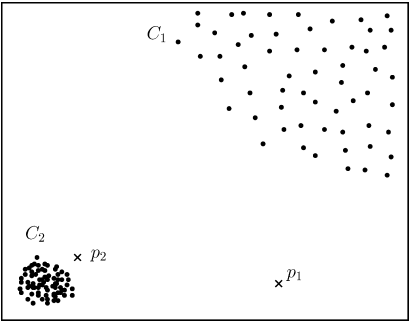
\includegraphics{chap01/localvsglobal.png}
	\caption{Result}
\end{figure}

\begin{itemize}
	\item \textbf{K-distance} :The distance between a data point p
	and its $K^{th}$ nearest neighbor (K-NN).
	
	\item \textbf{Reachability distance (reach-dist)} of a data point p
	with respect to another data point o
	
	\[ reach-dist_K(p,o)=max\{k-distance(o),d(p,o)\}  \]
	
	where d(p,o) is the euclidean distance between p
	and o.
	
	
	\item \textbf{Local Reachability Density(lrd)}  of a data point p
	
	
	\[  lrd_k(p) =  \bigg( \frac{1}{K} \sum_{o \in N_{(p,k)}} reach-dist(p,o)   \bigg)^{-1}  \]
	
	
	where $N_{(p,k)}$ is the set of k nearest neighbors of p.
	
	\item
	\textbf{Local Outlier Factor(LOF)}  of a data point p
	
	\[  LOF_K(p) = \frac{1}{K} \sum_{o \in N_{(p,k)}} \frac{lrd_K(o)}{lrd_K(p)}  \]
	
\end{itemize}

\par LOF is a score assigned to each instance that shows the degree of anomalous behavior. Instances inside a cluster have LOF value nearly equal to 1.


\section{Incremental Local Outlier Detection for Data Streams}
Incremental LOF for data streams refer to computation LOF score of newly added data points and updating the same for older data points. Outlier detection techniques are categorized into 4 types

\begin{enumerate}
	\item \textit{Statistical Approach} : the data points are typically modeled using a stochastic distribution, and points are labeled as outliers depending on their relationship with this model.
	
	\item \textit{Distance Based Approach} : detect outliers by computing distances among points.
	
	\item \textit{Profiling Methods} : Profiles of normal behavior is built and deviation from that are considered outliers.
	
	\item \textit{Model-based Approach} : First characterization of normal points using predictive models like neural networks and SVM. Deviation from these models are considered outliers.
	
	
\end{enumerate}

Static LOF algorithms can be applied to data stream is three ways. However thwese are computationally inefficient.

\begin{enumerate}
	\item \textit{Periodic LOF} : Static LOF is applied periodically on entire data set every time new data blocks are entered. The problem with such approach is that a data point which may be anomalous while added may not be detected as outlier later as many other points are added. they may create a cluster of their own and outliers will be missed. If LOF is computed each time a data point is added, the change is behavior can be detected at that moment.
	
	\item \textit{Supervised LOF} : K-distance, lrd and LOF of the data points are precomputed. Any new data point that arrives all these parameters are computed without updating for previous points. As a result the LOF accuracy decreases. 
	
	\item \textit{Iterated LOF} : Aplpy static LOF every time a new data point enters. This gives high accuracy at a cost of very high computational time. 
	
	
\end{enumerate} 

In Incremental approach, LOF score is computed as soon as a data enters. It is determined whether it is outlier or not. LOF of other data points are also updated. 

\subsection{Insertion}

K-distance, lrd, LOF are computed for each inserted data point and updated for affected points. 

\begin{algorithm}[h!]
	\caption{iLOF Insertion}
	\begin{algorithmic}
		\STATE  
		\STATE INPUT:  A data point $p_t$ at time t
		\STATE OUTPUT: LOF value LOF($p_t$)
		\STATE
		
		\STATE Compute KNN and K-distance of $p_t$
		
		\FOR {all o \in KNN($p_t$)}	
		
		\STATE Compute \texttt{reach-dist($p_t$,o)}
		
		\ENDFOR
		
		\STATE  $S_{update}$ \leftarrow Reverse KNNs of $p_t$
		
		\FOR{ all o \in $S_{update}$ and q \in $N_{(o,k)}$}
		
		\STATE Update K-distance(o) and reach-dist(q,o)
		
		\IF {o \in  $N_{(q,k)}$}
		
		\STATE $S_{update}$ \leftarrow  $S_{update}$ \cup q
		\ENDIF
		
		\ENDFOR
		
		\FOR { all o \in $S_{update}$ }
		
		\STATE Update lrd(o) and LOF(R-KNN(o,k))
		
		\ENDFOR
		\STATE Compute lrd($p_t$) and LOF($p_t$)
		\RETURN LOF
		
		
	\end{algorithmic}
\end{algorithm}


\section{Memory Efficient Incremental Local Outlier Factor (MiLOF)}

Local Outliers detection in data streams when limited memory is available. It is impractical to store all the instances of data streams. Some of the points has to be removed and summarized. Memory available is just sufficient to store K-Distance, lrd and LOF of m data points only.

The available m memory is divided in two parts of size b and c to store original points and summarized points respectively. When memory limit is reached, first ${\frac{b}{2}}$  data points are summarized to c clusters and deleted to free memory. If there already exists summarized data, the old and new cluster centers are merged. Hence at any time maximum memory used is b=m+c.
 Three steps of MiLOF are 

\subsection{Summarization}
Whenever memory reaches limit b, summarization phase is invoked. This phase summarizes first ${\frac{b}{2}}$ points, their K-distance, lrd and LOF and deletes these points from memory. Recent points are retained because data points might have evolved with time and recent points are most important. As the width of the summarization window decreases, it resembles iLOF. So MiLOF is direct generalization of iLOF.

\par 
Summarization  is explained in algorithm 2.
In summarization, if memory is reached first $\frac{b}{2}$ points are summarized to c clusters. K-distance, lrd and LOF for these cluster centers are computed by the following formulas.  

\begin{itemize}
	\item K-Distance of cluster center $v^i_j$ \in $V^i$ 
	
	
		\[  K-Distance(v^i_j) = \frac{\sum_{p \in C^i_j } K-Distance(p)}{| C^i |} \]
		
		
	 \item lrd of cluster center $v^i_j$ \in $V^i$ 
		
		
		\[  lrd_k(v^i_j) = \frac{\sum_{p \in C^i_j } lrd_k(p)}{| C^i |} \]
		
		\item LOF of cluster center $v^i_j$ \in $V^i$ 
		
		
		\[  LOF_k(v^i_j) = \frac{\sum_{p \in C^i_j } LOF_k(p)}{| C^i |} \]
	
\end{itemize}


\begin{algorithm}[h!]
	\caption{MiLOF}
	\begin{algorithmic}
		\STATE  
		\STATE INPUT:  A data point p 
		\STATE OUTPUT: LOF value LOF(p)
		\STATE
		
		\STATE Compute LOF of p 
		\IF {No of points=b}
			\STATE $C^i$ $\leftarrow$ First $\frac{b}{2}$ points
			\STATE ($V^i$,$N^i$) $\leftarrow$ C-means($C^i$)
			
			\FOR {all $v^i$ \in $V^i$} 
			  \STATE Compute avereage K-distance, lrd and LOF
			\ENDFOR
			
			\STATE Delete $C^i$
			
			\IF{i>0}
				\STATE (Z;W) $\leftarrow$ Weighted c-means($V^i$ U $V^{i-1}$ ,$N^i$ U $N^{i-1}$)
				
				\FOR {all z \in Z} 
					\STATE Compute avereage K-distance, lrd and LOF
				\ENDFOR 
				\STATE $V^{i-1}$ \leftarrow Z
				\STATE Delete $V^{i-1}$,Z
				
			\ENDIF	
		\ENDIF
		
		\STATE i $\leftarrow$ i+1
		\RETURN LOF
	\end{algorithmic}
\end{algorithm}

\subsection{Merging}

Summarization is performed every time new $\frac{b}{2}$ new data points arrives. Clustering these points gives c cluster centers $V^i$. These clusters are to be merged with old c cluster centers $V{i-1}$ so that finally only c centers are available. Cluster centers X={$V^i$ U $V^{i-1}$} are merged using a weighted clustering algorithm where weight of each center is no of objects in that cluster. 


\subsection{Revised Insertion}
Whenever a new data points arrives, LOF value for it is computed similar to iLOF with only difference that iLOF uses only data points to compute LOF where as in revised insertion we use both the data points and the cluster centers. While calculating the KNN, if any of the point is cluster center then it is assumed that all other nearest neighbor belongs to the same cluster. Hence distance from the point and that cluster center is taken as the K-distance for that point.  






\thispagestyle{empty}
\cleardoublepage
% % % % % % % % % % % % % % % % % % % % % % % % % % %
% % % % % % % % % % % % % % % % % % % % % % % % % % %
\chapter{Implementation and Results}\label{Implementation and Results}

\section{LOF}
We have used a synthetic 2-D dataset with 3 clusters of varying density to implement and verify LOF.
Dataset description\\
No of attributes : 2\\
No of instances  : 1500\\
No of clusters   : 3\\
Cluster 1        :  750 points in range [600,1000] \\
Cluster 2        :  500 points in range [200,450] \\
Cluster 3        :  200 points in range [0,100] \\
Noisy points	 : 50

\begin{figure}[h!]
	\centering
	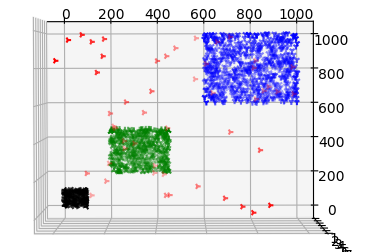
\includegraphics{chap03/LOF_dataset.png}
	\caption{2-D Dataset used for LOF}
\end{figure}

It can be seen from Figure 3.2 that points inside a cluster has LOF values nearly equal to 1 where as noisy points have LOF up to 7. More the LOF score more is the degree of anomaly.

\begin{figure}[h!]
	\centering
	\includegraphics{chap03/LOF_result.png}
	\caption{LOF values for synthetic 2-D dataset}
\end{figure}



  


\thispagestyle{empty}
\cleardoublepage
% % % % % % % % % % % % % % % % % % % % % % % % % % %
% % % % % % % % % % % % % % % % % % % % % % % % % % %
%%\section{Introduction}\label{Guidelines}
Submission of synopsis or extended abstract is one of the mandatory requirements before submitting a doctoral or master thesis. It is not just a longer version of an abstract. It is as good as a research paper that conveys the essence of the thesis without overlooking the importance of introduction and conclusion. A synopsis should include the following~\textemdash~
\begin{itemize}
	\item Introduction
	\item Aim
	\item Method
	\item Results
	\item Conclusion
	\item Limitations
	\item References
	\item Dissemination
\end{itemize}

\noindent A synopsis is a self-contained, capsule description of the thesis that must make sense all by itself. Typical length of a synopsis should be between 5 and 10. Pages must of A4 dimension with 25mm margin on all four sides. The entire dissertation must be written using only a single font including all the texts inside graphs, figures, block diagrams, etc. While writing captions of tables and figures, the font size should be decreased by one point. Similarly, the font size of bibliography and index should also be lessened by a point. Students are advised to use the following in the body text~\textemdash
\begin{itemize}
\item[] serif fonts like Times New Roman (TNR) of size 12pt \\
or \\
\textsf{sans-serif fonts like Arial of size 11pt}. 
\end{itemize}
Needless to say that the use of font should be uniform throughout. Headings, Titles \textit{etc.} should use fonts as given below in Table~\ref{tab-fonts}.
{
\linespread{1}
\begin{table}[h]
\centering
\caption{Font sizes to be used in the dissertation}
\begin{tabular}{l C{25mm} C{25mm} c} 
\toprule
{Item} & Arial & {TNR} & {Justification}\\
\midrule\midrule
Main Text & 11 normal & 12 normal & Justified \\
\midrule
Sub-sub Heading & 11 bold & 12 bold & Left \\
\midrule
Sub Heading & 13 bold & 14 bold & Left \\
\midrule
Heading$^{\#}$ & 16 bold & 17 bold & Left \\
\midrule
Chapter Title & 22 bold & 24 bold & Center \\
\midrule
Chapter Number & 16 bold & 17 bold & Left \\
\bottomrule
\multicolumn{4}{l}{$^{\#}$Add serial number with one decimal place.} 
\end{tabular}
\label{tab-fonts}
\end{table}
}
\par The class file \texttt{NITR.cls} can be used to prepare a synopsis. One needs to invoke the statement ``\texttt{\textbackslash synopsisCoverPage}'' in the main ``\texttt{.tex}'' file with ``\texttt{\textbackslash docType(4)}'' and all necessary data in the ``\texttt{FrontPages.tex}''. The text of the synopsis can be written in ``\texttt{./SynopsisText/SynopsisText.tex}''.
%%\thispagestyle{empty}
%%\cleardoublepage
%%% % % % % % % % % % % % % % % % % % % % % % % % % % %
%%% % % % % % % % % % % % % % % % % % % % % % % % % % %
\rhead{\textit{References}}
\lhead{}
\renewcommand\bibname{References}

%%%\bibliographystyle{Ref/IEEEtran}
\bibliographystyle{Ref/asme}
%%%\bibliographystyle{Ref/naturemag}
%%%\bibliographystyle{Ref/bmes}
%%%\bibliographystyle{Ref/achemso}
%%%\bibliographystyle{Ref/rsc}
%%%\bibliographystyle{Ref/osajnl}
%%
{
	\fontsize{10}{12}
	\selectfont
	\addcontentsline{toc}{chapter}{References}
	\bibliography{Ref/SampleReferences}
	\footnotetext{This reference format follows ASME style. You are advised to follow one reference format of any dominant journal of your field.}
}
\cleardoublepage
%%% % % % % % % % % % % % % % % % % % % % % % % % % % %
%%% % % % % % % % % % % % % % % % % % % % % % % % % % %
\rhead{\textit{Dissemination}}
\lhead{}
\SpecialTitle{Dissemination}


\paragraph{Internationally indexed journals} (\textit{Web of Science, SCI, Scopus, etc.})\footnote{\label{published}Articles already published, in press, or formally accepted for publication.}
\begin{itemize}
\item[1.]
\item[2.]
\end{itemize}  

\paragraph{Other journals and Book chapters}\footnotemark[\ref{published}]
\begin{itemize}
\item[1.]
\item[2.]
\end{itemize}  

\paragraph{Conferences}\footnotemark[\ref{published}]
\begin{itemize}
\item[1.]
\item[2.]
\end{itemize}  

\paragraph{Article under preparation}\footnote{\label{unpublished}Articles under review, communicated, or to be communicated.}
\begin{itemize}
\item[1.]
\item[2.]
\end{itemize}  
%
%\begin{itemize}
%\item[]\textbf{Internationally indexed journals}
%\item[1.]
%\item[2.]
%  
%\item[]
%
%\item[]\textbf{Conference Presentations}
%\item[1.]
%\item[2.]
%\item[]
%
%\item[]\textbf{Book Chapters}
%\item[1.]
%\item[2.]
%\end{itemize}

\thispagestyle{empty}
\cleardoublepage
% % % % % % % % % % % % % % % % % % % % % % % % % % %
% % % % % % % % % % % % % % % % % % % % % % % % % % %
\indexColumns{3}
\indexPage
% % % % % % % % % % % % % % % % % % % % % % % % % % %
% % % % % % % % % % % % % % % % % % % % % % % % % % %
\end{document}
